% Mantido pelo colegiado do curso de Bacharelado em Sistemas de informação do Centro Universitário Católica de Santa Catarina
% {juliano.marcelino,rodrigo.gregori}@catolicasc.org.br
% Este arquivo pode ser redistribuído e/ou modificado sobre a licença pública GNU versão 2.


\documentclass{beamer}

\usepackage[utf8]{inputenc}
\usepackage[T1]{fontenc}
\usepackage[brazil,english]{babel}
\usepackage{graphicx}

\usetheme{catolicasc}

\title{Paradigma Imperativo}

% Um subtítulo é opcional e pode ser comentado ou excluído


\author{\inst{}}
% - Indique os autores conforme o artigo ou sequência da apresentação.
% - Use o comando \inst{?} apenas se os autores tem diferentes afiliações.

\institute[Instituto Federal de Alagoas]
% opcional, mas normalmente mantido
{
  \inst{1}%
  Departamento de Sistemas de Informação\\
  Centro Universitário Católica de Santa Catarina em Jaraguá do Sul
  \and
  \inst{2}%
  Departamento de Sistemas de Informação\\
  Centro Universitário Católica de Santa Catarina em Jaraguá do Sul}
% - Use o comando \inst apenas se houver mais de uma afiliação.
% - Seja simples e objetivo, não há necessidade de colocar o endereço, cep, sala, etc

\date{Linguagem de Programação, 2018}
% - Coloque o nome da disciplina ou uma abreviação.
% - Serve para que pessoas de fora consigam entender o contexto da apresentação.

\subject{Assunto}
% Este campo permite mostrar o assunto no catálogo PDF, pode ser comentado ou removido (Propriedades do arquivo PDF).

% Desmarque o comentário apenas se quiser que a lista de tópicos apareça a cada nova subseção.
%\AtBeginSubsection[]
%{
%  \begin{frame}<beamer>{Outline}
%    \tableofcontents[currentsection,currentsubsection]
%  \end{frame}
%}

% E aqui começa o conteúdo de sua apresentação

\begin{document}

\begin{frame}
  \titlepage    
\end{frame}

\begin{frame}{Equipe}
    \begin{itemize}
        \item{Anderson Carlos}
        \item{Andre Luiz}
        \item{Carlos Eduardo}
        \item{Ginaldo Junior}
        \item{Izabel Helena}
    \end{itemize}
\end{frame}

\begin{frame}{Sumário}
  \tableofcontents
\end{frame}

% Seções e subseções vão aparecer automaticamente no slide Agenda, bem como a lista de conteúdos.
\section{Paradigma de Programação}
\subsection{O que é um paradigma?}


\begin{frame}{Paradigma de Programação}
    O que é um paradigma?
    \begin{itemize}
    \item{O paradigma de uma linguagem de programação é a sua identidade. Corresponde a um conjunto de características que, juntas, definem como ela opera e resolve os problemas. Algumas linguagens, inclusive, possuem mais de um paradigma, são as chamadas multi paradigmas.}
  \end{itemize}
\end{frame}

\section{Paradigma Imperativo}

\subsection{Origem}
\subsection{Arquitetura de Von Neumann}
\subsection{Funcionamento do Paradigma Imperativo}
\subsection{Características}

\begin{frame}{Paradigma Imperativo}
  \begin{itemize}
    \item{Programação imperativa é um paradigma de programação que descreve a computação como ações, enunciados ou comandos que mudam o estado de um programa.}
  \end{itemize}
\end{frame}

\begin{frame}{Paradigma Imperativo}
    Origem
    \begin{itemize}
      \item{Segunda Guerra Mundial}
      \item{O ENIAC tinha altos custos de manutenção e implementação} 
  \end{itemize}
  \begin{figure}
    \centering
    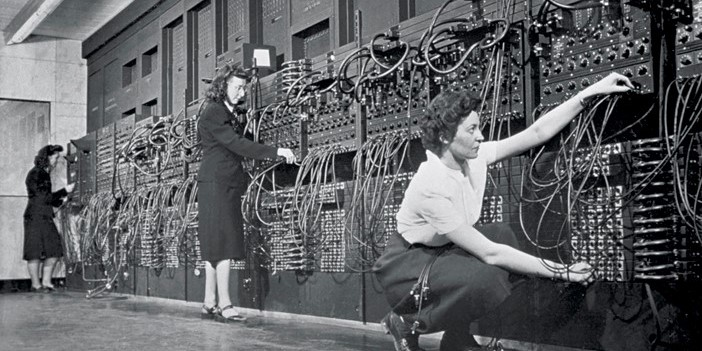
\includegraphics[scale=0.5]{eniac.jpg}
    \label{Rótulo}
  \end{figure}
\end{frame}

\begin{frame}{Paradigma Imperativo}
    Origem
    \begin{itemize}
        \item{Arquitetura de Von Neumann}
        \begin{itemize}
            \item{A Arquitetura de von Neumann é uma arquitetura de computador que se caracteriza pela possibilidade de uma máquina digital armazenar seus programas no mesmo espaço de memória que os dados, podendo assim manipular tais programas.}
        \end{itemize}
        \item{O Paradigma Imperativo é criado para suportar essa arquitetura}
    \end{itemize}
\end{frame}


\begin{frame}{Paradigma Imperativo}
Arquitetura de Von Neumann
  \begin{figure}
    \centering
    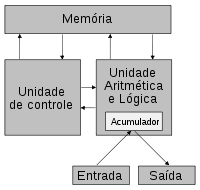
\includegraphics[scale=0.7]{von.png}
    \label{Rótulo}
  \end{figure}
\end{frame}

\begin{frame}{Paradigma Imperativo}
Funcionamento do Paradigma Imperativo
    \begin{figure}
            \centering
            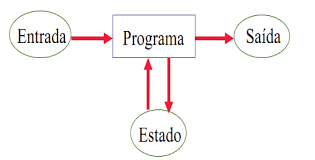
\includegraphics[scale=0.8]{paradigma.png}
            \label{Rótulo}
        \end{figure}
\end{frame}

\begin{frame}{Paradigma Imperativo}
Características
    \begin{itemize}
        \item{Atribuição, Declarações e Expressões}
        \item{Estruturas de controle}
        \item{Abstração procedural}
    \end{itemize}
\end{frame}



% Este tópico \appendix é opcional e pode ser removido se necessário.
\appendix
\section{\appendixname}
\subsection{Referências bibliográficas}

\begin{frame}[allowframebreaks]{Referências bibliográficas}

  \begin{thebibliography}{10}
    
  \beamertemplatearticlebibitems
  % Se usou livros, eis o exemplo

  \bibitem{Autor1990}
    Prof. Dr. Luiz Gustavo L. Fernandes
    \newblock Paradigmas de Linguagens de Programação
    \newblock https://www.inf.pucrs.br/~gustavo/disciplinas/pli/material/\\paradigmas-aula09.pdf.
 
    
  \beamertemplatearticlebibitems
  % Seguido de artigos principais usados

  \bibitem{Alguem2000}
    K.~Tedesco
    \newblock Linguagens e paradigmas de programação
    \newblock \em https://www.treinaweb.com.br/blog/linguagens-e-paradigmas-de-programacao 30/11/16
  \end{thebibliography}
\end{frame}

\end{document}